%--------------------------------------------------------------
\section{Documentação da \gls{api}}
%--------------------------------------------------------------
O Swagger, de acordo com sua documentação, é um \gls{framework} de código aberto que possui ferramentas que auxiliam na documentação dos serviços de uma \gls{REST API} com especificação \gls{openAPI}, o sistema deve apenas conter protocolos \acs{http} para aplicá-lo, independente da linguagem que está sendo utilizada. O Swagger realiza a descrição de todos os recursos da \acs{api}, mostrando quais métodos \acs{http}, entidades, operações possíveis e parâmetros a serem enviados de cada \textit{\glspl{endpoint}} da \gls{REST API}, por uma interface que a tecnologia disponibiliza, o Swagger UI. Portanto, este \gls{framework} facilita o entendimento do usuário em relação aos serviços de uma \acs{api}, proporcionando produtividade ao desenvolvedor.

Para a \acs{api} do projeto, está sendo utilizado a versão 3 do Swagger, pois esta versão é a mais atual e exige menos linhas de código para implementá-la, além de nos dar mais recursos, principalmente em relação à autenticidade do sistema, segundo sua documentação. O Swagger foi implementado através do arquivo \textit{pom.\acs{xml}}, sendo ele o é responsável por gerenciar as dependências do \gls{Maven}, após isso foi criada uma classe de configuração do \gls{SpringBoot} para geração da documentação \gls{openAPI} do sistema. A \autoref{swagger API} apresenta a interface do Swagger UI da \acs{api} desenvolvida.

\begin{figure}[htb]
\centering
\caption{\label{swagger API} Swagger UI da API}
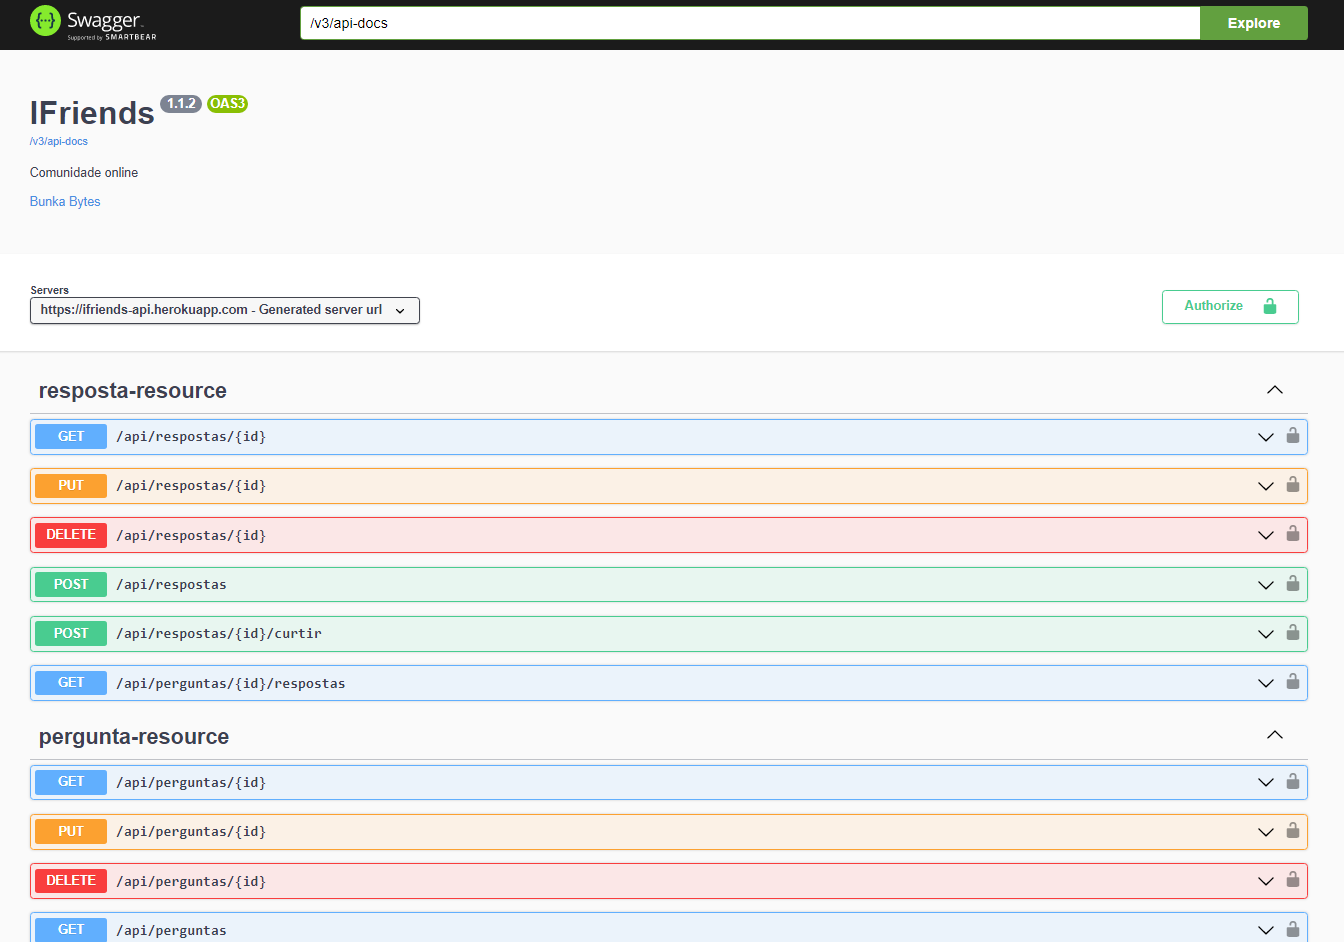
\includegraphics[width=1\textwidth]{anexos/Imagens_Swagger/API_swagger.png}
\fonte{Os autores}
\end{figure}
\FloatBarrier

Como foi possível constatar na \autoref{swagger API}, o canto superior da interface exibe informações gerais do projeto assim como o nome da \acs{api}, versão, descrição e nome da equipe. Já a parte central é mostrado o nome da classe de controle e a URI de cada requisição com seus métodos \acs{http}. O botão \textit{``Authorize''} possui a função de autenticar o usuário que está realizando a requisição através do \acs{jwt}. Após selecionar alguma requisição, é apresentado os parâmetros, o corpo da requisição e a descrição da resposta com o código de estado, como é possível observar na \autoref{demostracao swagger API}.

\begin{figure}[htb]
\centering
\caption{\label{demostracao swagger API} Exemplo Swagger na API}
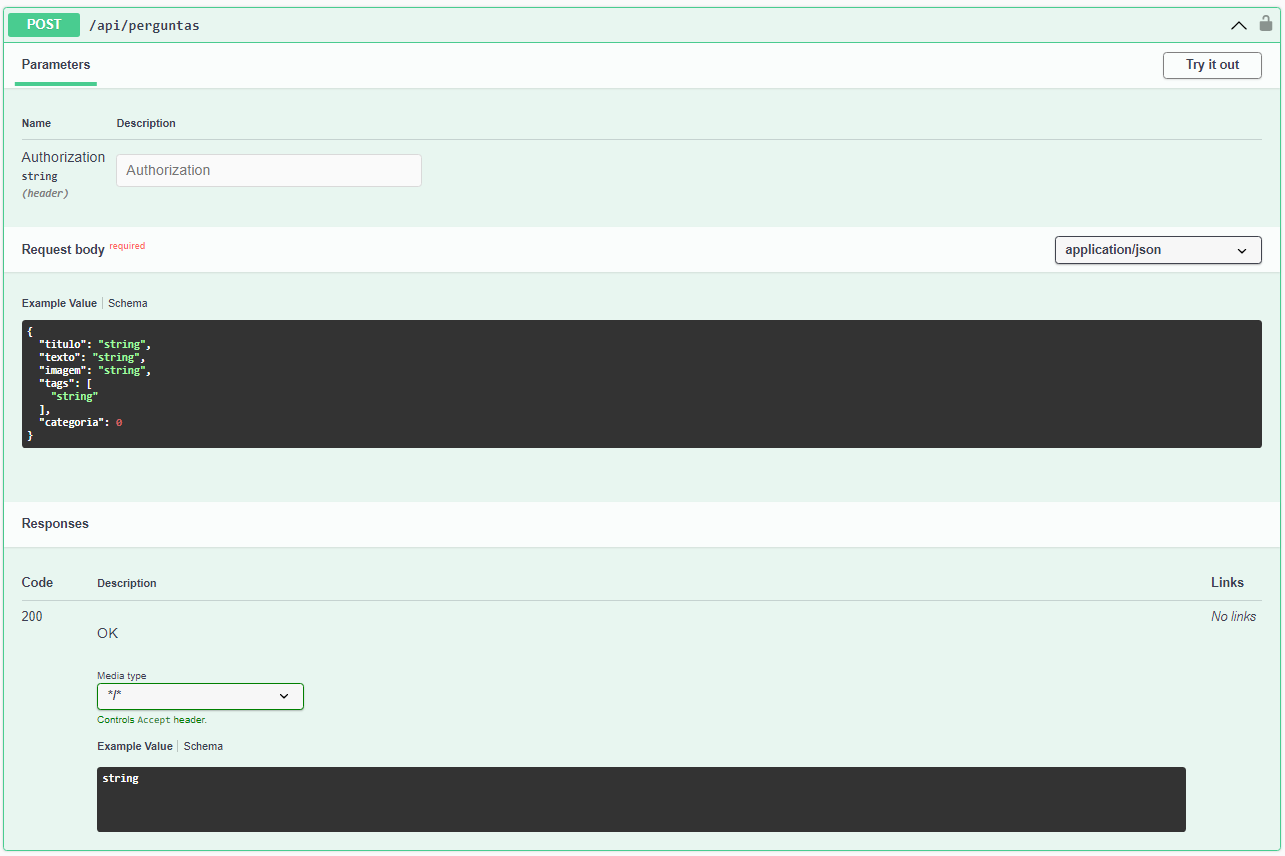
\includegraphics[width=1\textwidth]{anexos/Imagens_Swagger/API_swagger_demostracao.png}
\fonte{os autores}
\end{figure}
\FloatBarrier
